%%%%%%%%%%%%%%%%%%%%%%%%%%%%%%%%
% SECTION :: IR in our project %
%%%%%%%%%%%%%%%%%%%%%%%%%%%%%%%%
\section{IR in our project}
%%%%%%%%%%%%%%%%%%%%%%%%%%%%%%%%%%%
% Frame Open :: IR in our project %
%%%%%%%%%%%%%%%%%%%%%%%%%%%%%%%%%%%
\frame{\frametitle{IR in our project}
\begin{itemize}
\item Designing a good IR is more art than science.
\item Specially true in our project where there's only one source language
      (Poseidon) and one target language (MIPS).
\item In fact, do we really \textit{need} an IR in our project?
      Why not translate directly AST $\rightarrow$ MIPS?
\item For example, how should we translate \textit{32765+8}?
      (remember that addition is done with 16 bits overflow).
      One way is to handle the overflow in the AST $\rightarrow$ IR phase.
      Another way is to handle it during IR $\rightarrow$ MIPS phase.
      Which one is better?
\end{itemize}
\begin{figure}[htbp]
\begin{center}
% Requires \usepackage{graphicx}
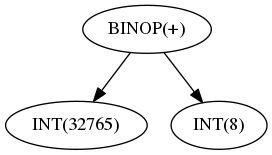
\includegraphics[width=4.0cm]{AST.png}\\
\label{Figure_Simple_Addition_Of_2_Integers_AST}
\end{center}
\end{figure}

%\centering
%\begin{tikzpicture}
%\tikzstyle{every node}=[draw,shape=circle];
%\node [text width=1cm, align=center] { Binop }
%child { node [text width=1cm, align=center] { Simple\\Var } }
%child { node [text width=1cm, align=center] {    INT(8)   } };
%\end{tikzpicture}
%%%%%%%%%%%%%%%%%%%%%%%%%%%%%%%%%%%
% Frame Close :: Warm up examples %
%%%%%%%%%%%%%%%%%%%%%%%%%%%%%%%%%%%
}